\chapter{Choosing the Test Radius around a DRP}
\label{choosingATestradius}
\index{Testradius!choosing a testradius}
In this section we discuss the choice of the so called "testradius" 
which is assigned to every Drive\_Route\_Point.
During this section, we assume that there is a fixed distance named $d$
between the Drive\_Route\_Points in question.
The distance $d$ is not measured directly ("as the crow flies") but 
along the path between the DRPs.

We do not discuss the choice of $d$ here, as this will be discussed in chapter~\ref{choosingDistance}.

%
% input: consideration for finding the maximal deflection
%
\section{Deflection from the direct Line}
\index{Deflection!Definition of}
\index{Deflection!Maximum Defection}
Given two DRPs $d_1$ and $d_2$  and a path between these points,
by "Deflection" we denote the maximum distance between the Path and the direct line between $d_1$ and $d_2$.
Figure \ref{pic:deflectionDefinition} illustrates the deflection of a path.
We will now discuss the "Maximum Deflection" from the direct line between to DRPs.
\begin{figure}[t]
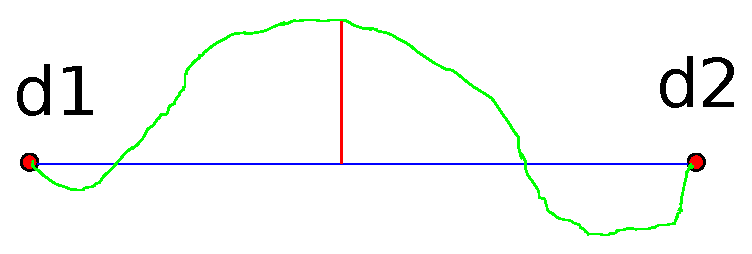
\includegraphics[scale=0.5]{images/03.01.deflection.eps}
\caption{Deflection of a path. The deflection (red) is defined as the maximum distance of the path (green) from the direct line (blue)}
\label{pic:deflectionDefinition} 
\end{figure}

\subsection{Maximum Deflection appears at Paths with \emph{exactly one} route point}
\label{Pathconstruction}

Keep in mind that a "Path" is composed of a finite number of RPs which are in turn connected by direct lines.
Given DRPs $d_1$ and $d_2$ and all paths of given length $d$ (and with arbitrary number of route points), 
we will now show that maximum deflection will appear at those paths which
have \emph{exactly one} route point.

More precisely, for every Path $P$ leading from $d_1$ to $d_2$ with RPs $rp_1,rp_2,.....,rp_n$ with deflection $h$ and length $d$, 
we can construct a path with $n-1$ routepoints and deflection $\tilde{h}$ \textgreater $h$ as follows:


\begin{enumerate}
	\item{From each triple of route points $rp_{j-1},rp_{j},rp_{j+1}$  where the three points are situated on
	      one direct line, eliminate the middle point $rp_{j}$. Note that this will not change the geometry of the path.
	      Iterate this process until there are no more three adjacent points on one line are left on the path.
	      }

	\item{From RPs $rp_1,rp_2,.....,rp_n$, chose an $rp_j$ such that the maximum deflection $h$ is realized at 
	      $rp_j$, and that there is one adjacent route point (wlog: $rp_{(j+1)}$}) such that
 	      the distance from $rp_{(j+1)}$ to the direct line between $d_1$ and $d_2$ is smaller than $h$.
	
	\item{Delete $rp_{j+1}$. Since there are no three points located on a line, the resuling path 
               $rp_1,rp_2,...,rp_j,rp_{j+2},..,rp_n$ is now shorter than the original path $rp_1,rp_2,.....,rp_n$
	      }

        \item{ It is now possible to replace $rp_j$ with a $\tilde{rp_j}$ further away from the direct line such that
	       the resulting Path  $\tilde{P}$ : $rp_1,rp_2,...,\tilde{rp_j},rp_{j+2},..,rp_n$ has length $d$,
	       and deflection greater than that of the original Path $P$, as desired. 	
	      }
\end{enumerate}

 
\begin{figure}[h]
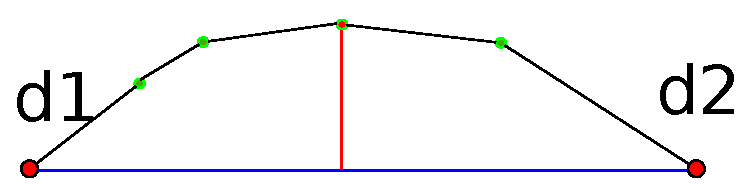
\includegraphics[scale=0.5]{images/03.02.deflection.eps}
\caption{Depicting construction in \ref{Pathconstruction}: 
	Original Path. Route point $r_j$ realizing the maximum deflection and maximum deflection
	in red.
	}
\end{figure}

\begin{figure}[h]
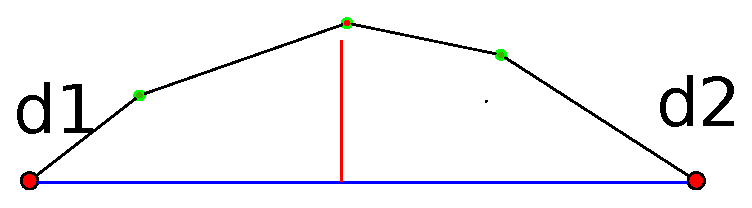
\includegraphics[scale=0.5]{images/03.03.deflection.eps}
\caption{
	Depicting construction in \ref{Pathconstruction}: 
	Route point $r_{j+1}$ now deleted. 
	Newly constructed RP $\tilde{rp_j}$ marked red.
	Original deflection marked by red line. 
	}
\end{figure}

\subsection{The Ellipse}
\index{Ellipse}

As a consequence of section \ref{Pathconstruction} we can now assume that a maximum deflection 
(maximal with respect to all paths of given length $d$) is realized by a Path with only one single RP. 
Given $d_1$ and $d_2$, and a fixed $d$ all the possible route points $rp$ have the common property
that the sum of the distances from $rp$ to $d_1$ and $d_2$ is $d$.
As this is exactly the defining property of the ellipse, all  $rp$ are located on an ellipse
with focal points $d_1$ and $d_2$.


\begin{figure}[h]
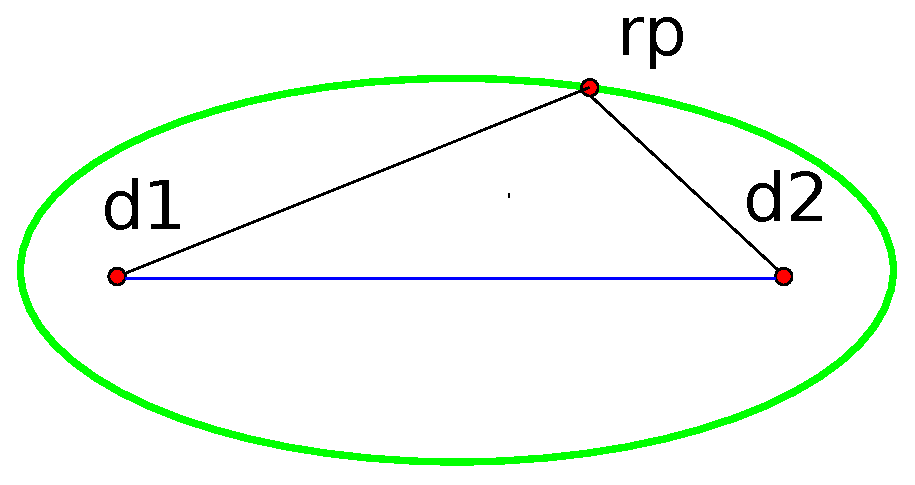
\includegraphics[scale=0.5]{images/03.04.ellipse.eps}
\caption{ For all paths with just one single route point $rp$ and with given length $d$,
	  all possible locations or $rp$ are located on an eclipse with focalpoints
	  $d_1$ and $d_2$	
	}
\end{figure}

\subsection{The Maximum Deflection as Function of the direct Distance between Drive\_Route\_Points}
\index{Direct Distance}
\index{Maximum Deflection!As function of the Direct Distance}
In view of the fact that an eclipse is symmetric, it becomes clear that for fixed $d$, the maximum
deflection becomes apparend exactly in the middle between $d_1$ and $d_2$.
With $\tilde{d}$ defined as the direct distance between $d_1$ and $d_2$, applying the Pythagorean Theorem,
the maximum deflection $h_{max}$ can be easily calculated to be:

\begin{equation}
 \label{HMaxOfD}  
 h_{max}(\tilde{d},d)=\sqrt{ \left(\frac{d}{2}\right)^2 - \left(\frac{\tilde{d}}{2}\right)^2 }
\end{equation}

Equation \ref{HMaxOfD} gives also an upper bound $h_{max}$ for $h_{max}(\tilde{d})$,
which is independent of $\tilde{d}$, and may be easier to calculate in some situations:

\begin{equation}
 \label{HMaxIndependent}  
 h_{max}=\frac{d}{2}
\end{equation}

Note also, that the independent bound in equation \ref{HMaxIndependent} is not completely unrealistic.
For example if points $d_1$ and $d_2$ are divided by some obstacle such as a railway or a river, then 
$\tilde{d}$ may come close to zero, and the bound in given in \ref{HMaxIndependent} gets realized.

\begin{figure}[h]
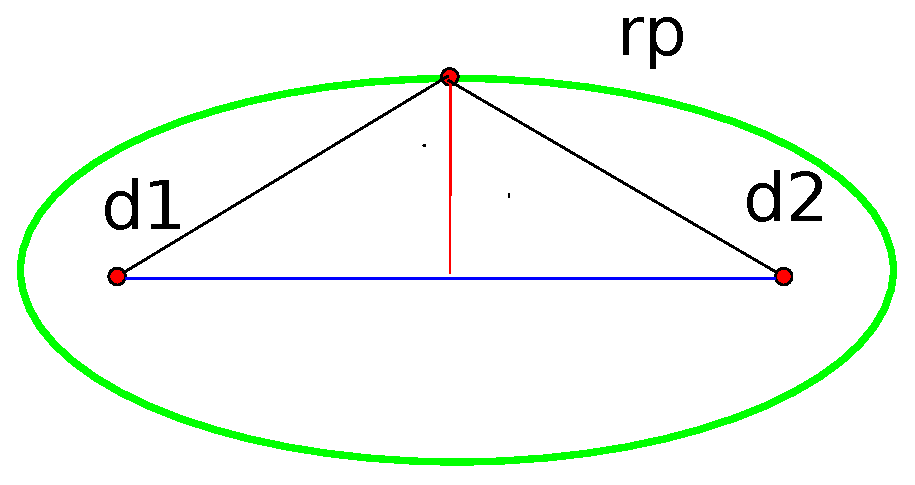
\includegraphics[scale=0.5]{images/03.05.formula.eps}
\caption{Depicting use of the Pythagorean Theorem to derive the formula for $h_{max}$: 
 	 $\frac{\tilde{d}}{2}$ (blue), $h_{max}$ (red) and $\frac{d}{2}$ form 
	 (two) rectangualar triangles
	}
\end{figure}










%
%
%
\section{The Testradius}
\index{Testradius}
\begin{figure}[h]
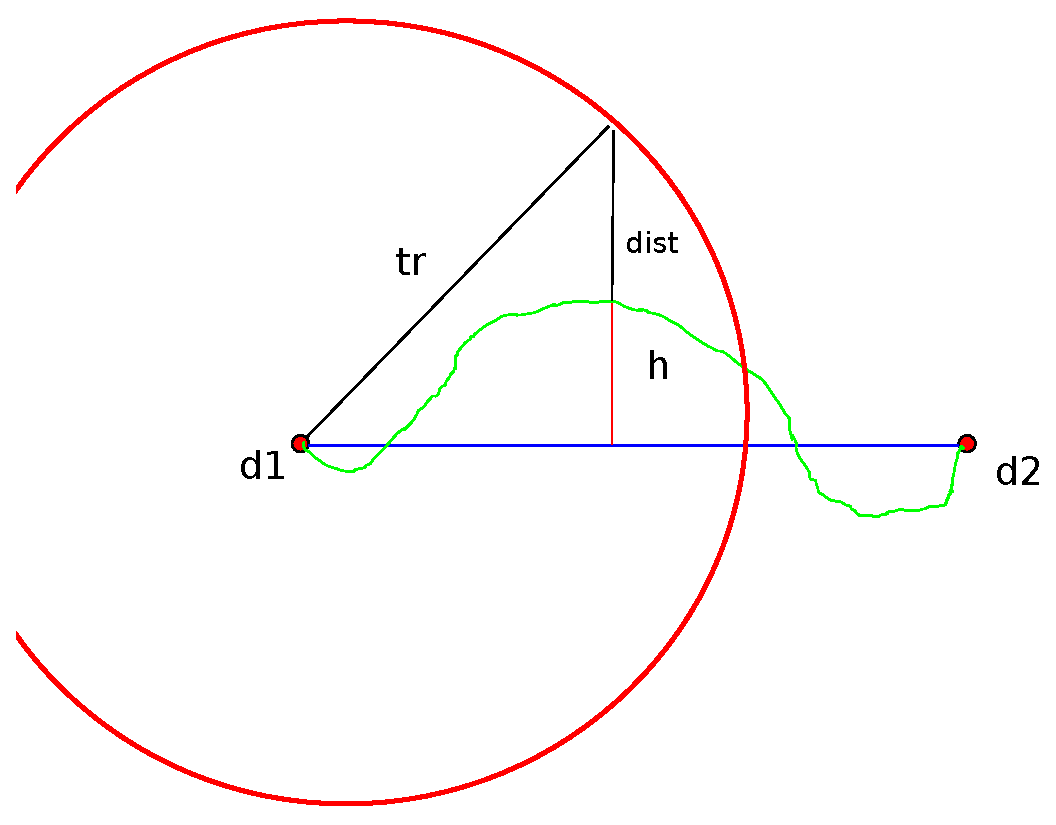
\includegraphics[scale=0.5]{images/03.06.testradius.eps}
\caption{Testradius $t_r$ must be large enough so that it covers any deflection $h$ \emph{plus} the user 
	 defined distance $dist$.
	}
\end{figure}

Summing up the results of the preceeding section, we now present formulas for calculating the 
test radius $t_r$.

We now consider two DRs $d_1$ and $d_2$ connected by a path $P$, with the distance from $d_1$ to $d_3$ beeing
$d$ along $P$ and $\tilde{d}$ in direct line. 
Assume further that P has a deflection $h$. By convexity we can assume this deflection to appear at the middle
of the line segment between $d_1$ and $d_2$. I.e: if the radius is large enough to cover the deflection
in the middle of the line segment, this deflection will be covered anywhere else.

Now the testradius $tr$ around $d_1$ must be large enough to cover a distance of $h+dist$ at a distance of $\frac{\tilde{d}}{2}$
from $d_1$.  The Phythagorean Theorem then gives the condition:
\index{Testradius!Condition for valid testradius} 
\begin{equation}
\label{testradius_condition}
 t_r^2  \geq \left(\frac{\tilde{d}}{2}\right)^2 + \left(h+dist\right)^2
\end{equation}

Condition \ref{testradius_condition} can be fulfilled with equality by choosing a radius $t_{r}$ as the square root of the right side:
\index{Testradius!Exact testradius tr}

\begin{equation}
 \label{testradius_general}
 t_r  := \sqrt{\left(\frac{\tilde{d}}{2}\right)^2 + \left(h+dist\right)^2}
\end{equation}

In practical application, it may turn out to be too tedious to calculate the exact deflection $h$ of 
the path $P$, so we can estimate the exact value $h$ by the upper bound $h_{max}(\tilde{d},d)$ 
from equation \ref{HMaxOfD}. 
This yields a larger valid testradius $t_{r1}$, which also fulfills \ref{testradius_general},
and has a more simple formula:   
\index{Testradius!approximation tr1}
\begin{equation}
 \label{testradius_tr1}
  t_{r1} := \sqrt{\left(\frac{\tilde{d}}{2}\right)^2 + \left(\sqrt{ \left(\frac{d}{2}\right)^2 - \left(\frac{\tilde{d}}{2}\right)^2 }+dist\right)^2}
\end{equation}

Not subtracting the term $\left( \frac{\tilde{d}}{2}\right)^2$ in the inner square root gives another  
valid choice $tr_2$ for a testradius:   
\index{Testradius!approximation tr2}
\begin{equation}
 \label{testradius_tr2}
  t_{r2} := \sqrt{\left(\frac{\tilde{d}}{2}\right)^2 + \left(\frac{d}{2}+dist\right)^2}
\end{equation}

Finally, as $ \tilde{d}$ is bounded by $ d $, a really simple formula for a valid
testradius $t_{r3}$  can be obtained, from  \ref{testradius_tr2},  
which does not even require calculation of the direct distance $\tilde{d}$:
\index{Testradius!approximation tr3}
\begin{equation}
 \label{testradius_tr3}
 t_{r3}  := \sqrt{ \frac{1}{2}d^2 + d*dist + dist^2}
\end{equation}



